\documentclass{article}

\usepackage[nonatbib,final]{neurips_2020}

\usepackage[utf8]{inputenc} % allow utf-8 input
\usepackage[T1]{fontenc}    % use 8-bit T1 fonts
\usepackage{hyperref}       % hyperlinks
\usepackage{url}            % simple URL typesetting
\usepackage{booktabs}       % professional-quality tables
\usepackage{amsfonts}       % blackboard math symbols
\usepackage{nicefrac}       % compact symbols for 1/2, etc.
\usepackage{microtype}      % microtypography
\usepackage{graphicx}
\usepackage{placeins}       % for \FloatBarrier
\usepackage[backend=biber,style=ieee,sorting=none]{biblatex}
\addbibresource{report.bib}

\title{Identification of microglia in mouse brain tissue using a convolutional 
neural network}

\author{
    Scott Howard
    \And
    Elliot Lupini
    \And
    Leo McKee-Reid
}

\begin{document}

\maketitle

\section{Introduction}

In order to better understand the brain and cure neurodegenerative diseases, 
neuroscientists image the brain to study its structure on a macro, cellular, 
and molecular scale. A common practice in cellular neuroscience is to use 
powerful microscopes to image very thinly sliced animal brain tissues that 
have been stained so that a specific cell stands out. As imaging technology 
improves, one of the bottlenecks in research has become the amount of image 
data that needs to be manually analyzed. In this project, we aim to replace the 
tedious process of manual cell identification by using a convolutional neural 
network (CNN) to detect microglia (a type of brain cell) in light microscopy 
images of mouse brain tissue. The image data we have used to train and test our 
model (see Figure \ref{fig:hippocampus}) has been provided by the Tremblay 
Lab --- a neuroscience lab at UVic with a research focus on microglia and how 
it impacts learning, stress, disease, and aging in the brain\parencite{tremblay}.

\begin{figure}[ht]
  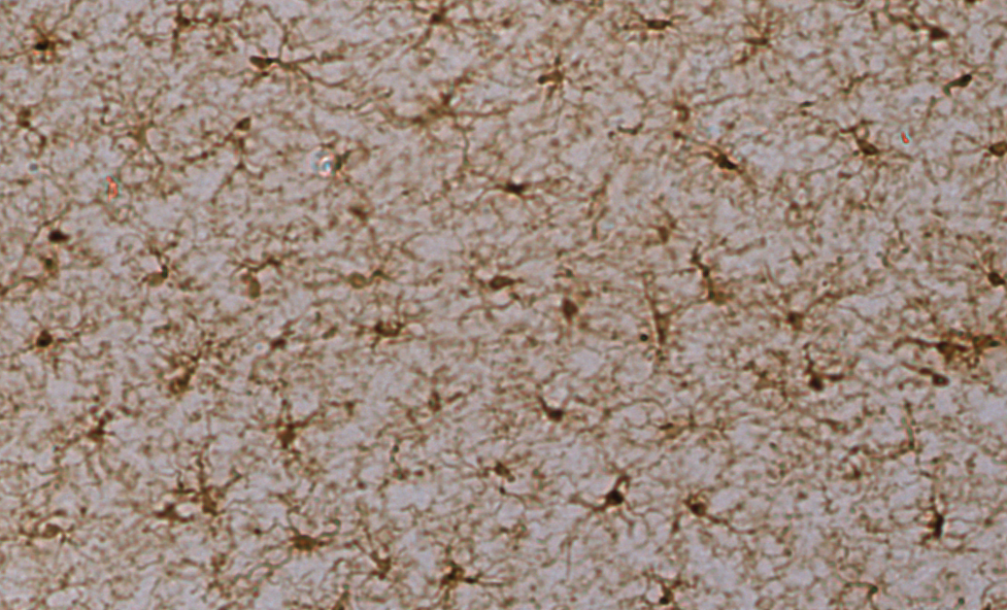
\includegraphics[width=0.7\textwidth]{hippocampus.png}
  \centering
  \caption{A slice of mouse brain tissue, imaged with light microscopy at the 
  Tremblay Lab. Most of the dark spots in the image are microglia cells---the 
  target of this experiment.}
  \label{fig:hippocampus}
\end{figure}

\section{The Problem}

The Tremblay Lab is currently researching how the density and distribution of 
microglia change in a mouse hippocampus. This requires researchers to 
manually label every microglia in tons of images, which both takes a lot of 
time and is sensitive to human error. To remove this research bottleneck, we 
have built a CNN that uses images that have already been manually annotated 
to generate the training and validation datasets for our model (see Figure 
\ref{fig:classification-dot}). Therefore, the input to our model is a raw, 
light microscopy image of a mouse hippocampus, and the output is the 
segmentation of the cell body.  Researchers in the lab can send this 
segmentation layer generated by the CNN into an image processing tool called 
ImageJ, which outputs the properly formatted density and distribution results 
they need.

The Tremblay Lab also wishes to build a similar CNN tool to do automatic 
morphology analysis. This is a much more challenging problem, as instead of 
simply identifying the center of each cell, it needs to trace around the cell 
body (i.e., segmentation) to determine the size and shape. The construction 
of this additional CNN is outside the scope of our project, however, since 
the model’s structure will be very similar to our cell identification CNN, we 
have built a testing metric for this morphology CNN. The work we have done in 
this project will therefore be the foundation for the morphology CNN, which 
will be trained and tested this summer. 

The formal goal of this project is therefore to train and test a CNN for 
microglia identification, and to develop the testing metric for the future 
morphology CNN.

\section{Background}

Object detection problems similar to this are common within computer vision 
(e.g., detecting a vehicle, a person, tumors, broken bones, etc.). The last 
decade has seen a large increase in neuroscience labs applying CNNs of this 
kind to cell detection and segmentation. There are also a few free, plug-and-
play software programs that do segmentation — such as Ilastik\parencite{ilastik}.
However, since the CNN models developed in other labs are fine-tuned to their 
datasets (and the fact that most labs are competing for funding and don't 
want to share their custom built tools), most neuroscience labs have to build 
their own CNNs. In addition, programs like Ilastik don’t yield a high enough 
testing accuracy unless the objects that are being classified really stand 
out from any other object in the image. For these reasons, the Tremblay Lab 
has decided to begin building their own CNN models, with our project being 
their first.

A CNN is a type of fully connected neural network that is commonly used for 
image classification. In order to recognize specific objects, a CNN 
simplifies an input image by applying convolutions (a type of filter) to 
create feature maps, which are then run through an activation function, and 
finally that output grid of pixels are pooled before sending the resulting 
pixel values into a neural network. Before training, these convolutions (which
are just an NxN grid of zeros or ones) are randomly generated. However, 
through backpropagation, the convolutions begin to change in order to 
minimize the error of the network’s prediction. This results in a set of 
convolutions that are finely tuned to produce the best predictions based on 
the training data.

Due to the way a CNN filters the input image, the best way to identify the 
center of microglia is to simply segment the cell body (since CNNs are good 
at finding the boundary of objects). This is the reason why our density and 
distribution CNN will be very similar to the post-project morphology CNN: 
they both have to trace out the cell body.

While segmentation software like Ilastik are not yet accurate enough for the 
data we’ve been provided, there are python libraries — such as
Gunpowder\parencite{gunpowder} and Pytorch\parencite{pytorch} --- that make 
the development of this type of model much easier. In the early stages of the 
project, we were able to use the model parameters from a Gunpowder tutorial 
that we were able to only minorly tweak in order to generate prediction 
images that qualitatively looked very accurate.

... blah blah blah, more info on the biology ...

This type of analysis is incredibly valuable, as it will increase our 
collective understanding of how microglia can contribute to, and fight against,
neurodegeneration. There are a number of projects in the lab that are already 
waiting to use our classification tool, and if this project is a success, 
publication of our results is quite likely.

\begin{figure}
  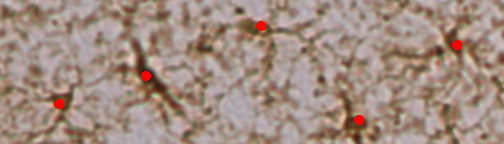
\includegraphics[width=0.7\textwidth]{classification-dot.png}
  \centering
  \caption{A cropped input image with manually labeled red dots to indicate where 
  the center of each microglia is.}
  \label{fig:classification-dot}
\end{figure}

\begin{figure}
  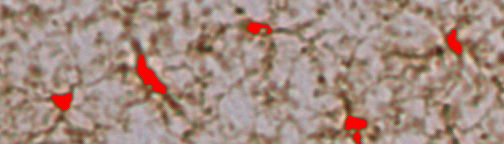
\includegraphics[width=0.7\textwidth]{classification-cell.png}
  \centering
  \caption{A cropped input image with manually labeled red dots to indicate where 
  the center of each microglia is.}
  \label{fig:classification-cell}
\end{figure}


\section{Method}

The approach we took can be broken down into 4 steps: preprocessing, training,
prediction, and post-processing. The microglia in the images that were given to
us by the Tremblay Lab were labeled with a single dot in the middle of the cell
body (see Figure \ref{fig:classification-dot}). However, our task 
required slightly different labeling (see Figure \ref{fig:classification-cell}),
so using ... we were able to easily transform the original single dots to 
cover the entire cell body. Now that we had the correct labels, we used 
Gunpowder to streamline the training/testing pipeline. This python library 
not only provides a clean pipeline, but also is advantageous for computer 
vision tasks. It allows for easy image manipulation as well as integrating 
with Pytorch. We needed to increase the size of our training set, so used 
Gunpowder to randomly sample the training images into smaller sizes as well 
as linearly transforming them to create more. The current parameters of our 
model are based on a Gunpowder tutorial, which implements a U-Net through a 
library interface to PyTorch. The predictions made by the model are passed 
through a post-processing routine to eliminate low pixel activations that 
correspond to "unconfident" predictions (see Figure ...).

\section{Results}

The benefit of a computer vision task is that we can qualitatively gauge how 
the model is performing, although quantitative measures are absolutely 
necessary to properly improve the predictions. Figure ... illustrates the 
output from the model alongside the raw image and ground truth. The 3rd row 
is the model’s prediction and the last row depicts the prediction after
post-processing. It’s important to see the output in order to properly understand 
the quantitative measures.

The results (see Figure ...) summarize the performance of better count and 
naive difference over all epochs. Each training epoch consisted of 720 images 
and then was tested on 19 images (larger size, but same resolution to not 
affect model performance). The count difference metric was normalized by the 
number of actual clusters in the image so the training and testing scores can 
be compared. Furthermore, the pixel difference metric was normalized by the 
size of the input image, which was 200x200 for the training dataset, and 
500x500 for the test dataset. The resulting value was the number of differing 
pixels, represented as a percentage.

\begin{table}
  \caption{Describe the table}
  \label{tbl:epoch-summary}
  \centering
  \begin{tabular}{ccrrr}
    \toprule
    epoch &  dataset & count difference & pixel difference (\%) \\
    \midrule
    01    & training &                7 &             1.97 \\
    02    & training &                5 &             0.98 \\
    03    & training &                6 &             1.09 \\
    04    & training &                6 &             1.04 \\
    05    & training &                6 &             1.04 \\
    06    & training &                6 &             1.04 \\
    07    & training &                6 &             1.02 \\
    08    & training &                5 &             0.94 \\
    09    & training &                6 &             1.11 \\
    10    & training &                5 &             0.97 \\
    11    & training &                8 &             1.29 \\
    \midrule
    01    &   test   &               32 &             3.42 \\
    02    &   test   &               12 &             1.48 \\
    03    &   test   &               24 &             3.26 \\
    04    &   test   &               33 &             3.52 \\
    05    &   test   &                9 &             1.07 \\
    06    &   test   &               11 &             1.98 \\
    07    &   test   &               14 &             3.08 \\
    08    &   test   &                6 &             1.86 \\
    09    &   test   &               10 &             2.62 \\
    10    &   test   &               27 &             2.16 \\
    11    &   test   &               15 &             1.78 \\
    \bottomrule
  \end{tabular}
\end{table}

After 11 epochs, the training count difference was 8, and the pixel 
difference was 1.29\%. The test count difference was 15, and the pixel 
difference was 1.78%.

\section{Discussion}

A significant barrier in this project was the time needed to train the model. 
Each epoch took approximately 1.5 hours meaning we were unable to run all the 
experiments we had hoped to. Parameter tuning becomes quite challenging when 
working with such complex data. Although Figure ... reveals inconsistent 
scores, it could be possible that this would appear to be a smooth, downward 
trend over 100 epochs. We are hopeful that we can use more sophisticated 
computing resources over the next couple weeks, but unfortunately didn’t have 
access leading up to this report.

What we can see though is that the model is overfitting, given that the 
training scores are much lower than the test scores. A main contributor to 
this is that the model is currently predicting a significant number of false 
positives. There are many dark spots in the raw images that are not microglia,
but the model is predicting them as positives. The first adjustment we would 
like to make would be to increase the penalty to predicting false positives. 
While ideally the model would be able to differentiate the dark spots from 
microglia, there is also the possibility that these false positives could be 
eliminated during post-processing. Analysis would need to be done to 
determine if, for example, the false predictions are much smaller than actual 
microglia, in which case if the cluster is below a certain size it could be 
eliminated.

\section{References}

\printbibliography[heading=none]

\end{document}
